% Activate the following line by filling in the right side. If for example the name of the root file is Main.tex, write
% "...root = Main.tex" if the chapter file is in the same directory, and "...root = ../Main.tex" if the chapter is in a subdirectory.

%!TEX root =  ../../Tesis.tex
\chapter{Modelos de barajado de secuencias}\label{anex:Modelos}

En el trabajo de investigaci�n que se recoge en el cap�tulo \ref{cap:Met} se desarrollaron distintos modelos computacionales con el objetivo com�n de obtener secuencias aleatorias de una frecuencia nucleot�dica igual a la de las secuencias reales (v�ase p�gina \pageref{sec:Modelos}). En la secci�n de Resultados del cap�tulo \ref{cap:Met} (p�gina \pageref{sec:Met:Resultados}) s�lo se incluyeron los resultados procedentes del barajado de secuencias mediante el modelo homog�neo, debido a que no se encontraron diferencias significativas entre los distintos modelos. En la figura \ref{figura:Modelos} se muestran los resultados que no fueron incluidos en el cuerpo de esta tesis.

% Figura Modelos
\begin{figure}[!htb]
\begin{center}
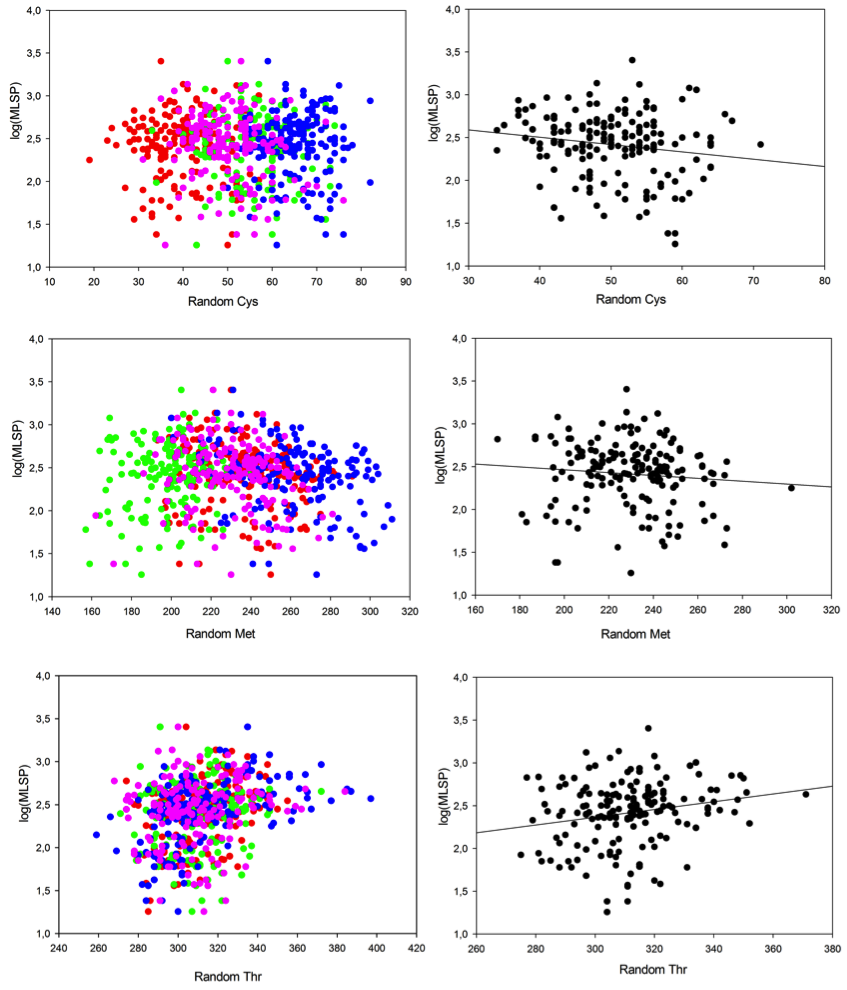
\includegraphics[width=1\textwidth]{Apendices/Modelos/Figuras/modelos.pdf}
\end{center}
\caption{\small{Influencia de la composici�n nucleot�dica sobre la abundancia de ciste�na, metionina y treonina en prote�nas codificadas por mtDNA. Para cada especie, se us� la secuencia, compuesta por los 12 genes concatenados de la hebra pesada, para generar otras secuencias aleatorias bajo los criterios de los distintos modelos, en los que cada posici�n de cada triplete es tratada como una categor�a independiente. Los c�rculos rojos, verdes y azules se corresponden con los modelos 1, 2 y 3, respectivamente. Los c�rculos p�rpuras representan los resultados obtenidos con el modelo 1-3. Por �ltimo, los c�rculos negros representan los resultados obtenidos con el modelo 1-2-3.}}
\label{figura:Modelos}
\end{figure}
% Fin de figura Modelos